\section{Data preprocessing} % ----------------------------------------------------+

\begin{figure}[ht!]
    \centering
        \subfloat{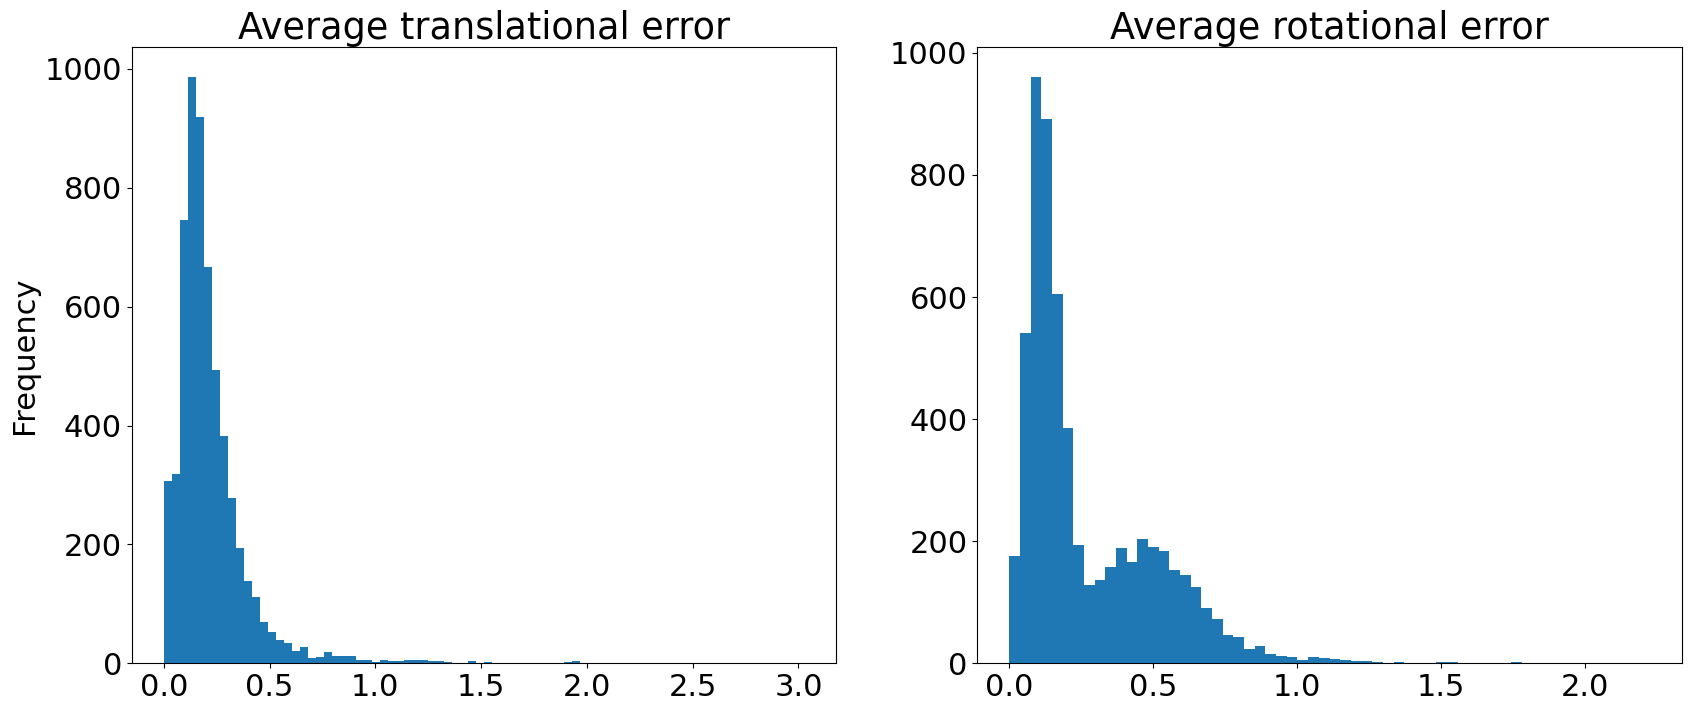
\includegraphics[width=.8\linewidth]{images/data_distribution.png}}
    \caption{Original localization error distribution}\label{fig:dataDistribution}
\end{figure}

\begin{figure}[ht!]
    \centering
        \subfloat{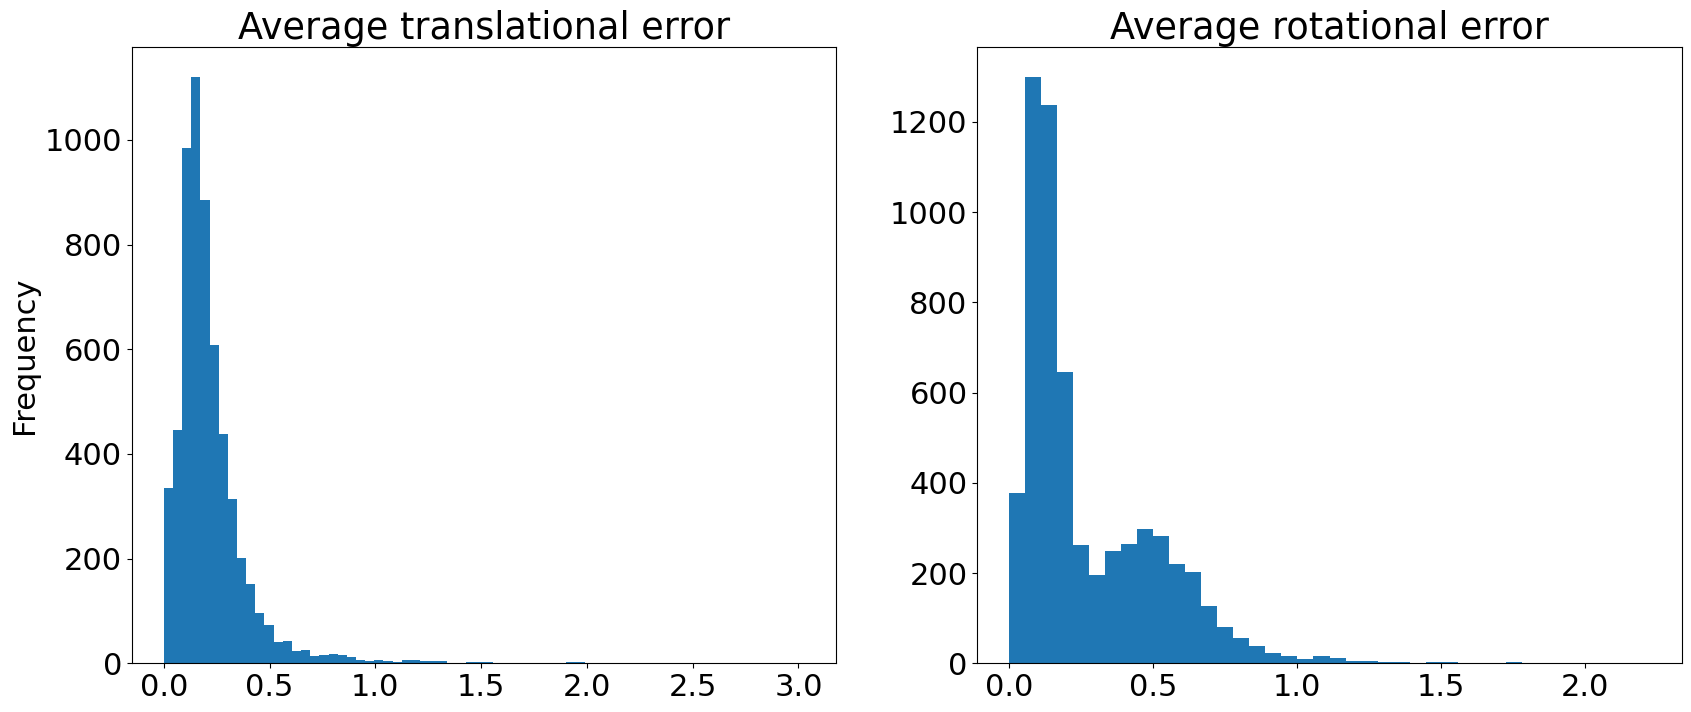
\includegraphics[width=.8\linewidth]{images/scaled_data.png}}
    \caption{Re-scaled localization errors}\label{fig:dataDistribution_scaled}
\end{figure}

\noindent
Both the ATE and ARE distributions exhibit right skewness, with the presence of a few outliers (Figure \ref{fig:dataDistribution}). To mitigate the effects of vanishing gradients and the influence of outliers, the data is scaled so that 99\% of the values fall between 0 and 1, as shown in Figure \ref{fig:dataDistribution_scaled}. Additionally, the area of each floorplan is normalized to the $[0, 1]$ range by dividing each datapoint by the maximum area value in the dataset.

% -----------------------------------------------------------
%                                                           \
%                                                           \
% -----------------------------------------------------------

\subsection{Image loading and dataset creation}\label{sec:dataset_creation} % ---------------------------------------
\noindent
Another preprocessing step consists in fixing images' resolution so that they can be fed to the CNN: for each floorplan we compute the minimum circumscribed square and scale it to a size \footnote{This resolution choice is rather generous, given that both CNNs internally re-scale the image to 224x224px. Storing the dataset at a higher resolution leaves some margin for future experiments with different models.} of 500x500px. 
Floorplan images are loaded and processed lazily using TensorFlow's \texttt{data} API\footnote{https://www.tensorflow.org/guide/data}, which handles automatically the allocation and de-allocation policies for the images. 

After splitting the floorplans in the usual train/validation/test partitions, respectively with 70/15/15 thresholds, the dataset creation steps consist of:
\begin{enumerate}
    \item Image loading.
    \item Data augmentation, which randomly rotates an image by multiples of 90°.
    \item Creation of each datapoint tuple \texttt{(image, area, label)}.
    \item Shuffling and batching of datapoints into mini-batches of size 64.
\end{enumerate}
Note that the data augmentation step is applied at runtime only on the training set, in order to improve the model generalization capabilities.
